\chapter{Specifikacija programske potpore}
		
	\section{Funkcionalni zahtjevi}	
			
			\noindent \textbf{Dionici:}
			
			\begin{packed_enum}
				
				\item Građani
				\item Zaposlenici				
				\item Administratori
				
			\end{packed_enum}
			
			\noindent \textbf{Aktori i njihovi funkcionalni zahtjevi:}
			
			
			\begin{packed_enum}
				\item  \underbar{Neregistrirani/neprijavljeni korisnik (inicijator) može:}
				
				\begin{packed_enum}
					
					\item se registrirati u sustav, stvoriti novi korisnički račun kao građanin ili zaposlenik
					\begin{packed_enum}
						
						\item  građanima je potrebno ime, prezime, adresa(ulica, kućni broj, mjesto), e-mail adresa, korisničko ime i lozinka
						\item  zaposlenima je potrebno korisničko ime i lozinka
						
					\end{packed_enum}
					
					\item vidjeti informacije o uslugama
					
						\begin{packed_enum}
						
						\item pretraživati naziv/kategoriju proizvoda
						\item popis dostupnih odlagališta s informacijama o odlagalištu (vrsta otpada, radno vrijeme)
						\item termine odvoza otpada za određenu lokaciju
						\item informacije o poduzeću koje zbrinjava otpad kao i njegove kontakt podatke
						
						\end{packed_enum}
					
					
				\end{packed_enum}
				
				\item \underbar{Građanin (inicijator) može:}
				
				\begin{packed_enum}
					
					\item vidjeti informacije o uslugama
					
					\begin{packed_enum}
						
						\item pretraživati naziv/kategoriju proizvoda
						\item popis dostupnih odlagališta u blizini mjesta stanovanja s informacijama o odlagalištu (vrsta otpada, radno vrijeme)
						\item termine odvoza otpada za određenu lokaciju
						\item informacije o poduzeću koje zbrinjava otpad kao i njegove kontakt podatke
						
					\end{packed_enum}
					
					\item napraviti zahtjeve prema poduzeću 
					
					\begin{packed_enum}
						
						\item izbor vrste i broj komada resursa za odlaganje(vrećice, kante, kontejneri) – potrebno                                obrazloženje uz zahtjev
						\item za odvozom krupnoga otpada - obrazloženje uz zahtjev
						\item ispis zahtjeva u pdf formatu		 		
						
					\end{packed_enum}
					
					\item slati pritužbu poduzeću koja sadrži naslov i opis, koju može ispisati u pdf formatu
					\item imati uvid u odgovor zaposlenika za svaki zahtjev i pritužbu ako postoji
					
				\end{packed_enum}
				
				\item \underbar{Zaposlenik (inicijator) može:}
				
				\begin{packed_enum}
					
					\item odgovarati na pritužbe i zahtjeve građanina
					\item brisati pritužbe i zahtjeve u suprotnosti s pravilima korištenja aplikacije
					\item izmijeniti informacije o:  
					
					\begin{packed_enum}
						
						\item prikladnim resursima za određeni proizvod
						\item odlagalištima
						\item terminima odvoza
						
					\end{packed_enum}
					
				\end{packed_enum}
				
				\item \underbar{Administrator (inicijator) može:}
				
				\begin{packed_enum}
					
					\item  vidjeti popis svih registriranih korisnika i njihovih osobnih podataka
					\item  brisati korisnike
					
					\item izmijeniti informacije o:
					
					\begin{packed_enum}
						\item prikladnim resursima za određeni proizvod
						\item odlagalištima
						\item terminima odvoza
					\end{packed_enum} 
					
				\end{packed_enum}	
				
				\item  \underbar{Baza podataka (sudionik):}
				
				\begin{packed_enum}
					
					\item pohranjuje sve: 
						
						\begin{packed_enum}
							
							\item podatke o korisnicima i zaposlenicima te njihovim ovlastima
							\item pritužbe i zahtjeve korisnika te odgovore na iste
							\item podatke o odlagalištima, terminima odvoza i resursima
							
							
						\end{packed_enum}
					
				\end{packed_enum}
			\end{packed_enum}
			
			\eject 
			
			
				
			\subsection{Obrasci uporabe}
				
				
				\subsubsection{Opis obrazaca uporabe}
					

					\noindent \underbar{\textbf{UC1 -Registracija građana}}
					\begin{packed_item}
	
						\item \textbf{Glavni sudionik: }Građanin
						\item  \textbf{Cilj:} Stvoriti korisnički račun za pristup sustavu
						\item  \textbf{Sudionici:} Baza podataka
						\item  \textbf{Preduvjet:} -
						\item  \textbf{Opis osnovnog tijeka:}
						
						\item[] \begin{packed_enum}
	
							\item Građanin odabire opciju za registraciju
							\item Građanin unosi ime, prezime, adresu stanovanja, adresu e-pošte, korisničko ime i lozinku
							\item Građanin prima obavijest o uspješnoj registraciji
						\end{packed_enum}
						
						\item  \textbf{Opis mogućih odstupanja:}
						
						\item[] \begin{packed_item}
	
							\item[2.a] Odabir postojećeg korisničkog imena ili e-maila, unos korisničkih podataka u nevaljalom formatu ili unos nepostojećeg emaila
							\item[] \begin{packed_enum}
								
								\item Sustav obavještava korisnika o neuspjeloj registraciji i vraća ga na stranicu za registraciju. Građanin mijenja nevaljale podatke ili odustaje od registracije.
								
								
							\end{packed_enum}

							
						\end{packed_item}
					\end{packed_item}
				
				
				\noindent \underbar{\textbf{UC2 -Prijava u sustav}}
				\begin{packed_item}
					
					\item \textbf{Glavni sudionik: }Registrirani korisnik
					\item  \textbf{Cilj:} Dobiti pristup korisničkom sučelju
					\item  \textbf{Sudionici:} Baza podataka
					\item  \textbf{Preduvjet:} Registracija
					\item  \textbf{Opis osnovnog tijeka:}
					
					\item[] \begin{packed_enum}
						
						\item Korisnik unosi korisničko ime i lozinku
						\item Potvrda o ispravnosti unesenih podataka
						\item Pristup korisničkim funkcijama
					\end{packed_enum}
					
					\item  \textbf{Opis mogućih odstupanja:}
					
					\item[] \begin{packed_item}
						
						\item[2.a] Unos nepostojećeg korisničkog imena/lozinke
						\item[] \begin{packed_enum}
							
							\item Sustav obavještava korisnika o neuspjelom upisu i vraća ga na stranicu za prijavu
							
						\end{packed_enum}
						
						
					\end{packed_item}
				\end{packed_item}
			
			\noindent \underbar{\textbf{UC3 -Pretraživanje otpada}}
			\begin{packed_item}
				
				\item \textbf{Glavni sudionik: }Građanin
				\item  \textbf{Cilj:} Pretraživanje naziva ili kategorije proizvoda koji se razvrstava, za koji se navodi tip resursa za dozvoljeno odlaganje
				\item  \textbf{Sudionici:} Baza podataka
				\item  \textbf{Preduvjet:} Građanin je prijavljen
				\item  \textbf{Opis osnovnog tijeka:}
				
				\item[] \begin{packed_enum}
					
					\item Građanin odabire opciju  "Vrste otpada"
					\item Građanin pretražuje otpad po imenu ili kategoriji
					\item Prikaže se tip resursa za dozvoljeno odlaganje (određeni tip vrećice, tip kante ili kontejnera) i slika istoga
				\end{packed_enum}
				
				\item  \textbf{Opis mogućih odstupanja:}
				
				\item[] \begin{packed_item}
					
					\item[2.a] Za pretraživani naziv ili kategoriju proizvoda koji se razvrstava ne postoji informacija u sustavu
					\item[] \begin{packed_enum}
						
						\item Sustav obavještava građanina o nedostupnosti informacija za zatraženi naziv ili kategoriju
						
					\end{packed_enum}
					
					
				\end{packed_item}
			\end{packed_item}
		
			\noindent \underbar{\textbf{UC4 -Pregled obližnjih odlagališta}}
			\begin{packed_item}
				
				\item \textbf{Glavni sudionik: }Građanin
				\item  \textbf{Cilj:} Informiranje korisnika o dostupnim odlagalištima otpada u blizini njegove adrese stanovanja
				\item  \textbf{Sudionici:} Baza podataka
				\item  \textbf{Preduvjet:} Građanin je prijavljen
				\item  \textbf{Opis osnovnog tijeka:}
				
				\item[] \begin{packed_enum}
					
					\item Građanin odabire opciju "Obližnja odlagališta"
					\item Građaninu se prikazuju obližnja odlagališta otpada 
					\item Građanin odabire odlagalište koje ga zanima
					\item Otvara se Google Maps i lokacija odlagališta, te sve informacije o odlagalištu (vrste podržanog otpada, radno vrijeme)
				\end{packed_enum}
			\end{packed_item}
			
			\noindent \underbar{\textbf{UC5 -Pregled termina odvoza otpada}}
			\begin{packed_item}
				
				\item \textbf{Glavni sudionik: }Građanin
				\item  \textbf{Cilj:} Saznati termine odvoza otpada za određenu lokaciju
				\item  \textbf{Sudionici:} Baza podataka
				\item  \textbf{Preduvjet:} Građanin je prijavljen 
				\item  \textbf{Opis osnovnog tijeka:}
				
				\item[] \begin{packed_enum}
					\item Građanin odabire opciju "Termini odvoza"
					\item Građaninu se prikazuju termini odvoza kućnog otpada za njegovu adresu stanovanja
				\end{packed_enum}
			\end{packed_item}

				\noindent \underbar{\textbf{UC6 -Informacije o poduzeću za odvoz otpada}}
				\begin{packed_item}
					
					\item \textbf{Glavni sudionik: }Građanin
					\item  \textbf{Cilj:}Pregled informacija o poduzeću koje zbrinjava otpad
					\item  \textbf{Sudionici:} Baza podataka
					\item  \textbf{Preduvjet:} Građanin je prijavljen
					\item  \textbf{Opis osnovnog tijeka:}
					
					\item[] \begin{packed_enum}
						
						\item Pregled informacija o poduzeću koje zbrinjava otpad koje uključuje kontakt-informacije
					\end{packed_enum}
				\end{packed_item}
			
				\noindent \underbar{\textbf{UC7 -Zahtjev za dodatnim resursima za odlaganje otpada }}
				\begin{packed_item}
					
					\item \textbf{Glavni sudionik: }Građanin
					\item  \textbf{Cilj:} Slanje zahtjeva za dodatnim resursima za prikupljanje kućnog otpada
					\item  \textbf{Sudionici:} Baza podataka
					\item  \textbf{Preduvjet:} Građanin je prijavljen
					\item  \textbf{Opis osnovnog tijeka:}
					
					\item[] \begin{packed_enum}
						\item Građanin odabire opciju "Zahtjev za dodatnim resursima"
						\item Odabire resurs za odlaganje
						\item Piše obrazloženje zašto zahtijeva dodatne resurse
						\item Prima potvrdu o uspješno poslanom zahtjevu
						\item Građanin ima mogućnost iskrcavanja zahtjeva u obliku PDF-a na lokalno računalo
					\end{packed_enum}
					
					\item  \textbf{Opis mogućih odstupanja:}
					
					\item[] \begin{packed_item}
						
						\item[2.a] Slanje zahtjeva bez obrazloženja
						\item[] \begin{packed_enum}
							
							\item Sustav upozorava građana da mora napisati obrazloženje
							\item Građanin piše obrazloženje ili odustaje od slanja zahtjeva
							
						\end{packed_enum}
						
						
					\end{packed_item}
				\end{packed_item}
				
				\noindent \underbar{\textbf{UC8 -Zahtjev za odvoz krupnog otpada }}
				\begin{packed_item}
					
					\item \textbf{Glavni sudionik: }Građanin
					\item  \textbf{Cilj:} Slanje zahtjeva za odvozom krupnog otpada
					\item  \textbf{Sudionici:} Baza podataka
					\item  \textbf{Preduvjet:} Građanin je prijavljen
					\item  \textbf{Opis osnovnog tijeka:}
					
					\item[] \begin{packed_enum}
						\item Građanin odabire opciju "Zahtjev za odvoz krupnog otpada"
						\item Šalje zahtjev za odvoz krupnog otpada sa svoje adrese stanovanja
						\item Dobiva potvrdu o zaprimljenom zahtjevu i datum odvoza
						\item Građanin ima mogućnost iskrcavanja zahtjeva u obliku PDF-a na lokalno računalo
					\end{packed_enum}
				\end{packed_item}
								
				\noindent \underbar{\textbf{UC9 -Stvaranje PDF-a }}
				\begin{packed_item}
					
					\item \textbf{Glavni sudionik: }Građanin
					\item  \textbf{Cilj:} Stvaranje PDF-a na temelju poslanog zahtjeva ili pritužbe
					\item  \textbf{Sudionici:} Baza podataka
					\item  \textbf{Preduvjet:} Zahtjev za odvoz krupnog otpada ili slanje pritužbe je poslan
					\item  \textbf{Opis osnovnog tijeka:}
					
					\item[] \begin{packed_enum}
						
						\item Sustav zaprima zahtjev za stvaranje PDF-a na temelju poslanog zahtjeva ili pritužbe
						\item Sustav stvara PDF i vraća ga naručitelju
					\end{packed_enum}
					
					\item  \textbf{Opis mogućih odstupanja:}
				\end{packed_item}
			
				\noindent \underbar{\textbf{UC10 -Slanje pritužbe}}
				\begin{packed_item}
					
					\item \textbf{Glavni sudionik: }Građanin
					\item  \textbf{Cilj:} Slanje pritužbe vezane za uslugu odvoza otpada i upravljanja otpadom
					\item  \textbf{Sudionici:} Baza podataka
					\item  \textbf{Preduvjet:} Građanin je prijavljen
					\item  \textbf{Opis osnovnog tijeka:}
					
					\item[] \begin{packed_enum}
						\item Građanin odabire opciju "Pošalji pritužbu"
						\item Piše pritužbu i šalje ju
						\item Dobiva potvrdu o zaprimljenoj pritužbi
						\item Građanin ima opciju iskrcati pritužbu u formatu PDF-a na lokalno računalo
					\end{packed_enum}
					
					\item  \textbf{Opis mogućih odstupanja:}
					
					\item[] \begin{packed_item}
						
						\item[2.a] Slanje prazne pritužbe
						\item[] \begin{packed_enum}
							
							\item Sustav obavještava korisnika o neuspjelom zaprimanju prazne pritužbe
							\item Građanin piše pritužbu ili odustaje od slanja pritužbe
							
						\end{packed_enum}
						
						
					\end{packed_item}
				\end{packed_item}
			
				\newpage
			
				\noindent \underbar{\textbf{UC11 -Registracija zaposlenika}}
				\begin{packed_item}
					
					\item \textbf{Glavni sudionik: }Zaposlenik
					\item  \textbf{Cilj:} Stvoriti račun zaposlenika za pristup sustavu
					\item  \textbf{Sudionici:} Baza podataka
					\item  \textbf{Preduvjet:} Zaposlenik je evidentiran u sustavu kao radnik
					\item  \textbf{Opis osnovnog tijeka:}
					
					\item[] \begin{packed_enum}
						
						\item Zaposlenik odabire opciju za registraciju
						\item Zaposlenik unosi ime, prezime, adresu e-pošte, korisničko ime i lozinku
						\item Zaposlenik prima obavijest o uspješnoj registraciji
					\end{packed_enum}
					
					\item  \textbf{Opis mogućih odstupanja:}
					
					\item[] \begin{packed_item}
						
						\item[2.a] Odabir postojećeg korisničkog imena ili e-maila, unos podataka u nevaljalom formatu ili unos nepostojećeg emaila
						\item[] \begin{packed_enum}
							
							\item Sustav obavještava korisnika o neuspjeloj registraciji i vraća ga na stranicu za registraciju
							\item Zaposlenik mijenja nevaljale podatke ili odustaje od registracije
							
						\end{packed_enum}
						
						
					\end{packed_item}
				\end{packed_item}
			
				\noindent \underbar{\textbf{UC12 -Odgovaranje na zahtjeve za dodatnim resursima}}
				\begin{packed_item}
					
					\item \textbf{Glavni sudionik: }Zaposlenik
					\item  \textbf{Cilj:} Obrada zahtjeva građana za dodatnim resursima
					\item  \textbf{Sudionici:} Baza podataka
					\item  \textbf{Preduvjet:} Zaposlenik je prijavljen i postoji barem jedan neobrađen zahtjev za dodatnim resursima
					\item  \textbf{Opis osnovnog tijeka:}
					
					\item[] \begin{packed_enum}
						
						\item Zaposlenik odabire opciju "Zahtjevi za dodatnim resursima"
						\item Dobiva pregled svih neobrađenih zahtjeva i odabire jedan
						\item Na temelju obrazloženja odlučuje prihvaća li se zahtjev ili ne
						\item Odgovara građanu i zatvara zahtjev
					\end{packed_enum}
					
					\item  \textbf{Opis mogućih odstupanja:}
				\end{packed_item}
			
				\noindent \underbar{\textbf{UC13 -Odgovaranje na pritužbe građana}}
				\begin{packed_item}
					
					\item \textbf{Glavni sudionik: }Zaposlenik
					\item  \textbf{Cilj:} Odgovoriti na pritužbe građana
					\item  \textbf{Sudionici:} Baza podataka
					\item  \textbf{Preduvjet:} Zaposlenik je prijavljen i postoji barem jedna neobrađena pritužba
					\item  \textbf{Opis osnovnog tijeka:}
					
					\item[] \begin{packed_enum}
						
						\item Zaposlenik odabire opciju "Pritužbe"
						\item Dobiva pregled svih neobrađenih pritužbi i odabire jednu
						\item Odgovara na pritužbu i zatvara pritužbu
					\end{packed_enum}
				\end{packed_item}
			
				\noindent \underbar{\textbf{UC14 -Izmjena informacija o resursima za zbrinjavanje otpada}}
				\begin{packed_item}
					
					\item \textbf{Glavni sudionik: }Zaposlenik
					\item  \textbf{Cilj:} Izmijeniti / dodati informacije o resursima za zbrinjavanje otpada
					\item  \textbf{Sudionici:} Baza podataka
					\item  \textbf{Preduvjet:} Zaposlenik je prijavljen i postoji resurs koji želi izmijeniti
					\item  \textbf{Opis osnovnog tijeka:}
					
					\item[] \begin{packed_enum}
						
						\item Zaposlenik odabire opciju "Uređivanje informacija o resursima za odvoz"
						\item Dobiva pregled svih resursa za zbrinjavanje otpada i odabire jedan od njih
						\item Mijenja željene podatke i zaključava promjene
						\item Ako želi dodati novi resurs za zbrinjavanje otpada odabire opciju "Dodaj"
						\item Unosi sve potrebne podatke i zaključava unos
					\end{packed_enum}
					
					\item  \textbf{Opis mogućih odstupanja:}
					
					\item[] \begin{packed_item}
						
						\item[2.a] Kod stvaranja novog resursa za zbrinjavanje otpada ne unosi sve obavezne podatke
						\item[] \begin{packed_enum}
							
							\item Sustav obavještava zaposlenika o neuspjelom unosu i vraća ga na stranicu za dodavanje resursa
							\item Zaposlenik unosi obavezne podatke ili odustaje od dodavanja novog resursa
							
						\end{packed_enum}
						
						
					\end{packed_item}
				\end{packed_item}
			
				\noindent \underbar{\textbf{UC15 -Izmjena lokacija odlagališta }}
				\begin{packed_item}
					
					\item \textbf{Glavni sudionik: }Zaposlenik
					\item  \textbf{Cilj:} Izmijeniti / dodati informacije o odlagalištima otpada
					\item  \textbf{Sudionici:} Baza podataka
					\item  \textbf{Preduvjet:} Zaposlenik je prijavljen i postoji lokacija koju želi izmijeniti
					\item  \textbf{Opis osnovnog tijeka:}
					
					\item[] \begin{packed_enum}
						
						\item Zaposlenik odabire opciju "Uređivanje informacija o odlagalištima otpada"
						\item Dobiva pregled svih odlagališta i odabire jedno od njih
						\item Mijenja željene podatke i zaključava promjene
						\item Ako želi dodati novo odlagalište odabire opciju "Dodaj"
						\item Unosi sve potrebne podatke i zaključava unos
					\end{packed_enum}
					
					\item  \textbf{Opis mogućih odstupanja:}
					
					\item[] \begin{packed_item}
						
						\item[2.a] Kod stvaranja novog odlagališta ne unosi sve obavezne podatke
						\item[] \begin{packed_enum}
							
							\item Sustav obavještava zaposlenika o neuspjelom dodavanju novog odlagališta i vraća ga na stranicu za dodavanje odlagališta
							\item Zaposlenik unosi obavezne podatke ili odustaje od dodavanja novog odlagališta
							
						\end{packed_enum}
						
						
					\end{packed_item}
				\end{packed_item}
			
				\noindent \underbar{\textbf{UC16 -Izmjena termina odvoza otpada}}
				\begin{packed_item}
					
					\item \textbf{Glavni sudionik: }Zaposlenik
					\item  \textbf{Cilj:} Izmijeniti / dodati termine odvoza otpada
					\item  \textbf{Sudionici:} Baza podataka
					\item  \textbf{Preduvjet:} Zaposlenik je prijavljen i postoji termin koji želi izmijeniti
					\item  \textbf{Opis osnovnog tijeka:}
					
					\item[] \begin{packed_enum}
						
						\item Zaposlenik odabire opciju "Uređivanje termina za odvoz otpada"
						\item Dobiva pregled svih termina za odvoz i odabire jedan od njih
						\item Mijenja željene podatke i zaključava promjene
						\item Ako želi dodati novi termin odabire opciju "Dodaj"
						\item Unosi sve potrebne podatke i zaključava unos
					\end{packed_enum}
					
					\item  \textbf{Opis mogućih odstupanja:}
					
					\item[] \begin{packed_item}
						
						\item[2.a] Kod stvaranja novog termina ne unosi sve obavezne podatke
						\item[] \begin{packed_enum}
							
							\item Sustav obavještava zaposlenika o neuspjelom unosu i vraća ga na stranicu za dodavanje termina
							\item Zaposlenik unosi obavezne podatke ili odustaje od dodavanja novog termina
							
						\end{packed_enum}
						
						
					\end{packed_item}
				\end{packed_item}
			
				\noindent \underbar{\textbf{UC17 -Pregled svih korisnika}}
				\begin{packed_item}
					
					\item \textbf{Glavni sudionik: }Administrator
					\item  \textbf{Cilj:} Pregled svih registriranih građana i zaposlenika
					\item  \textbf{Sudionici:} Baza podataka
					\item  \textbf{Preduvjet:} Administrator je prijavljen
					\item  \textbf{Opis osnovnog tijeka:}
					
					\item[] \begin{packed_enum}
						
						\item Administrator odabire opciju "Pregled svih korisnika"
						\item Dobiva pregled svih registriranih građana i zaposlenika
					\end{packed_enum}
				\end{packed_item}
			
				\newpage
				
				\noindent \underbar{\textbf{UC18 -Brisanje korisnika}}
				\begin{packed_item}
					
					\item \textbf{Glavni sudionik: }Administrator
					\item  \textbf{Cilj:} Obrisati registrirani građanski račun ili zaposlenika
					\item  \textbf{Sudionici:} Baza podataka
					\item  \textbf{Preduvjet:} Administrator je prijavljen i postoji korisnički račun koji želi obrisati
					\item  \textbf{Opis osnovnog tijeka:}
					
					\item[] \begin{packed_enum}
						
						\item Administrator odabire opciju "Obriši korisnika"
						\item Unosi korisničko ime korisnika kojega želi obrisati
						\item Otvara se korisnički račun i otvara se potvrda za brisanjem računa
						\item Administrator briše korisnika ili odustaje od brisanja
					\end{packed_enum}
					
					\item  \textbf{Opis mogućih odstupanja:}
					
					\item[] \begin{packed_item}
						
						\item[2.a] Nepostojeće korisničko ime koje je administrator upisao
						\item[] \begin{packed_enum}
							
							\item Sustav obavještava administratora o nepostojećem korisniku
							
						\end{packed_enum}
						
						
					\end{packed_item}
				\end{packed_item}	
				\eject
				

				\subsubsection{Dijagrami obrazaca uporabe}
				
				\begin{figure}[H]
					\centering
					\includegraphics[width=\linewidth]{dijagrami/građani}
					\caption[Građani]{Dijagram obrasca uporabe, funkcionalnost građana i registriranog korisnika}
					\label{fig:graani}
				\end{figure}
				\begin{figure}
					\centering
					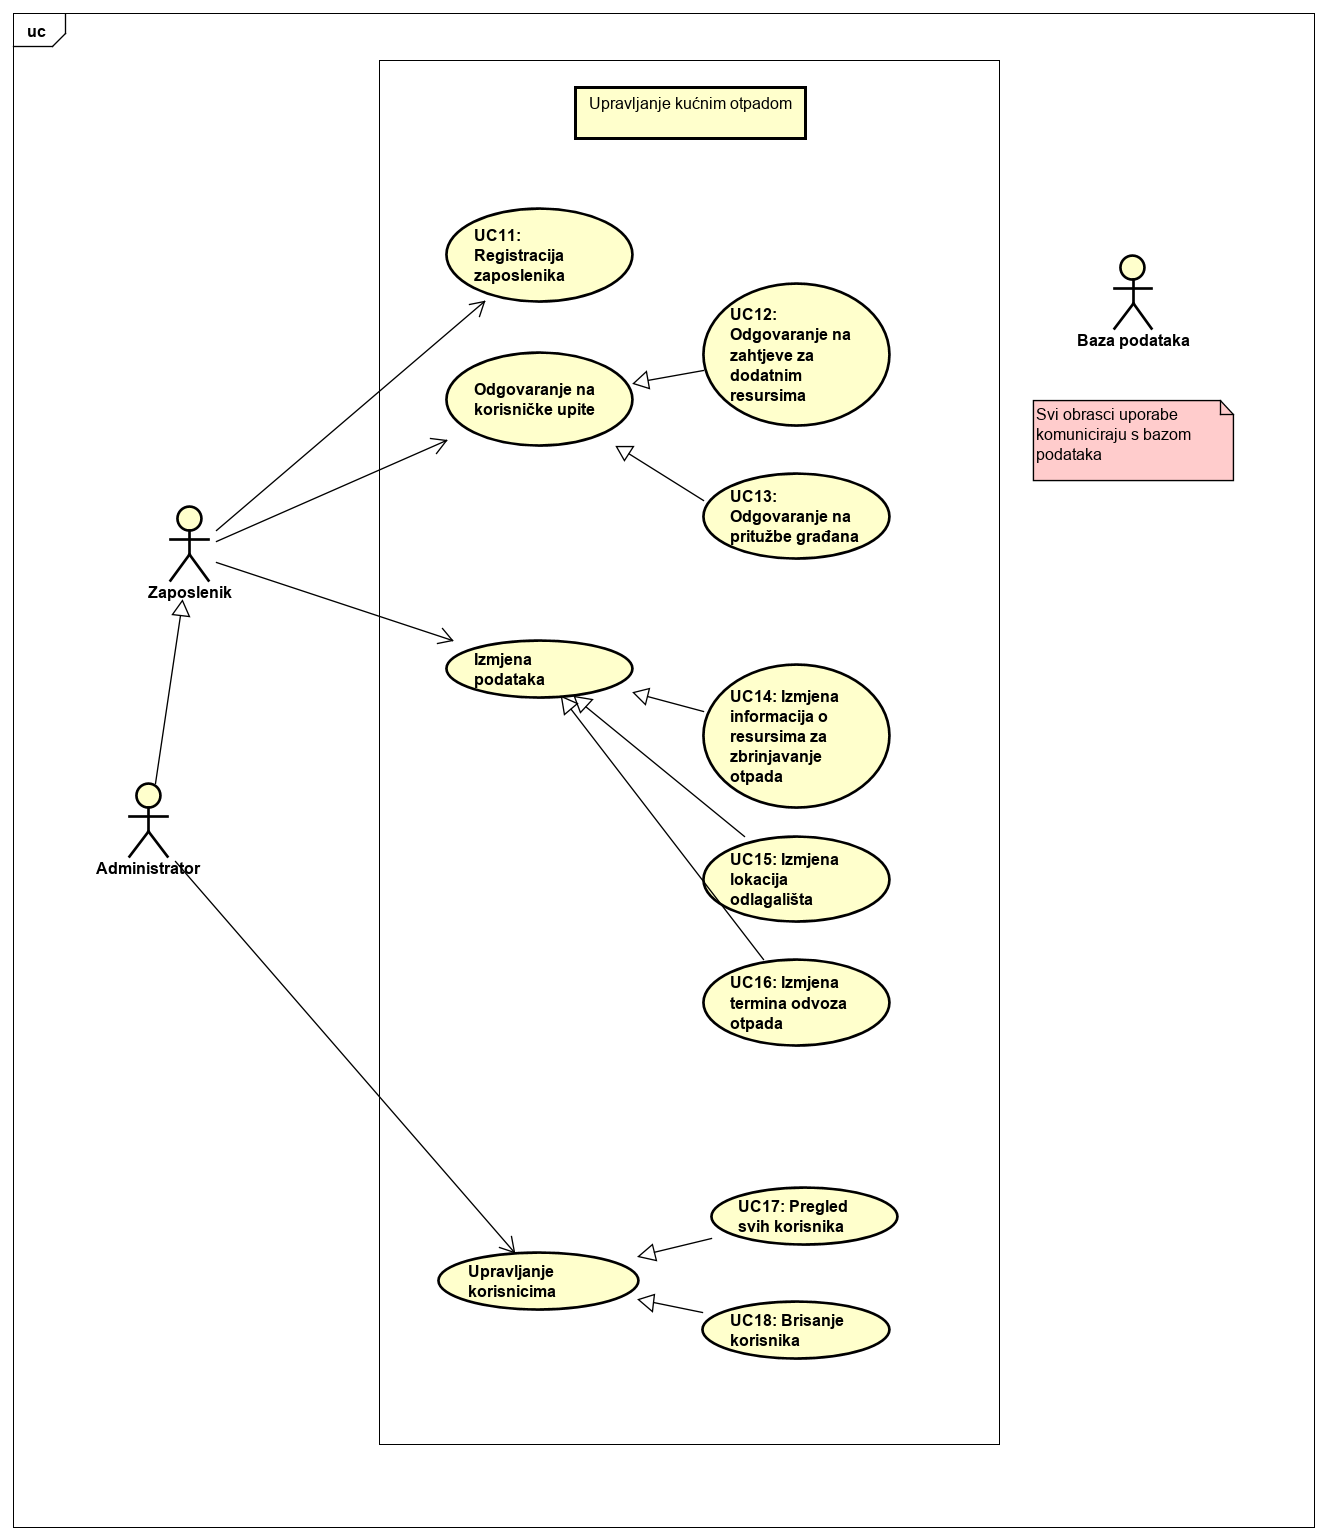
\includegraphics[width=1\linewidth]{dijagrami/zaposlenici}
					\caption[Građani]{Dijagram obrasca uporabe, funkcionalnost zaposlenika i administratora}
					\label{fig:zaposlenici}
				\end{figure}
			
				
				\eject
							
				
			\subsection{Sekvencijski dijagrami}
				
				
				
					\noindent {\textbf{Obrazac uporabe UC4 - Pregled obližnjih odlagališta}}
				\\
				
						\textmd{\textmd}{Klijent šalje zahtjev za pregled odlagališta u blizini svoje adrese stanovanja. Poslužitelj dohvaća najbliža odlagališta za otpad i prikazuje ih. Odabirom odlagališta, poslužitelj iz baze podataka dohvaća osnovne podatke o odlagalištu (vrsta otpada, radno vrijeme, kontakt...) i otvara lokaciju u Google Maps-u.}
						
					\begin{figure}[H]
						\centering
						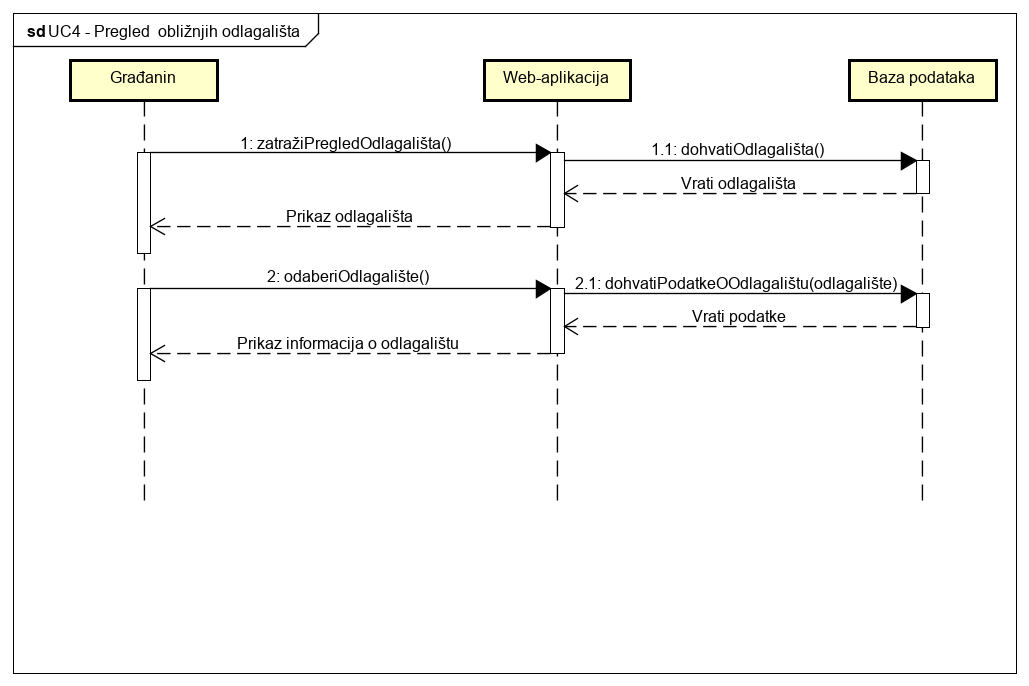
\includegraphics[width=\linewidth]{dijagrami/uc4seq}
						\caption{Sekvencijski dijagram za UC4}
						\label{fig:uc4seq}
					\end{figure}
				\newpage
				
				
				
				\noindent {\textbf{Obrazac uporabe UC18 - Brisanje korisnika}}
				\\
				
				\textmd{\textmd}{Administrator upisuje korisničko ime koje želi izbrisati. Poslužitelj dohvaća željenog korisnika i prikazuje sve korisničke podatke. Administrator tada potvrđuje svoju akciju brisanja. Ako ne postoji korisnik s upisanim korisničkim imenom poslužitelj o tome obavještava administratora. }
				\begin{figure}[H]
					\centering
					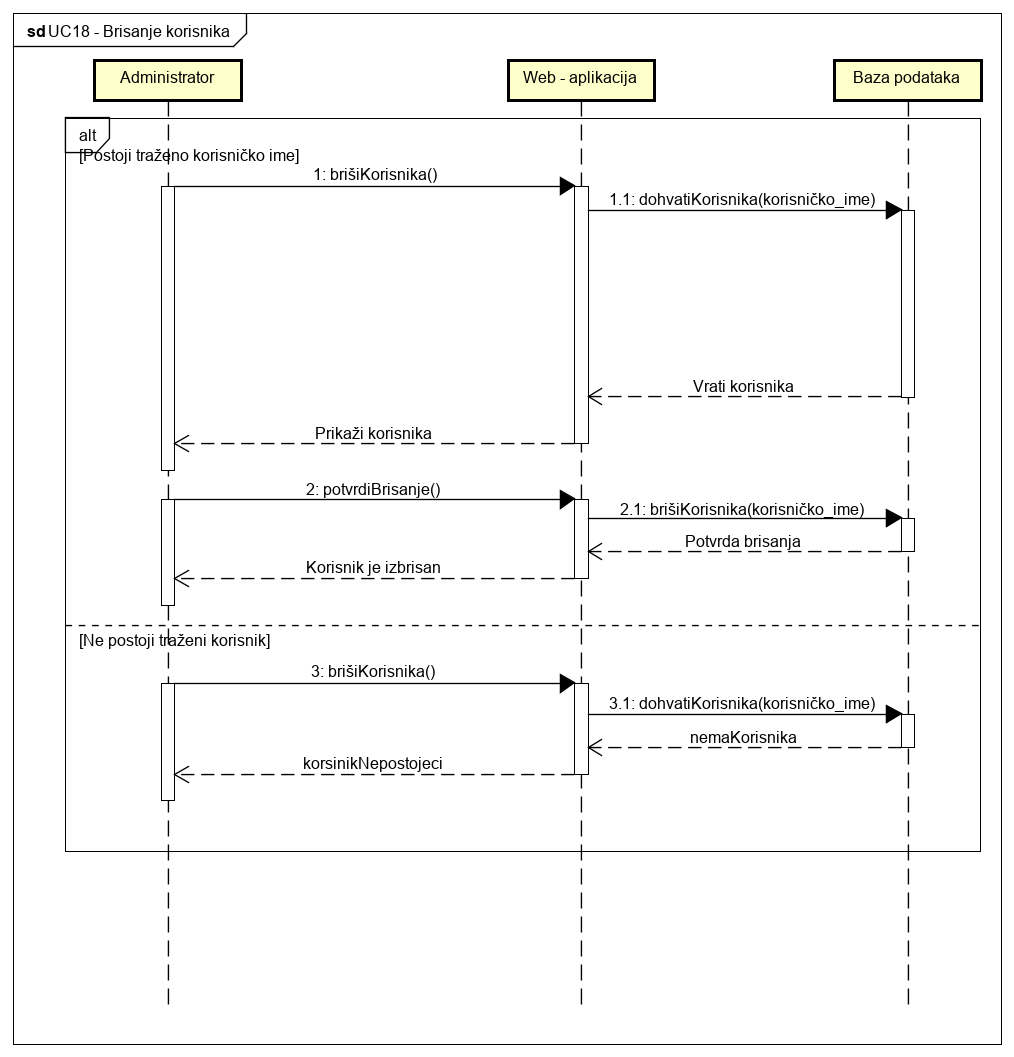
\includegraphics[width=1\linewidth]{dijagrami/brisanjeSeq}
					\caption{Sekvencijski dijagram za UC18}
					\label{fig:brisanjeseq}
				\end{figure}
			
			\eject
			
			

			\noindent {\textbf{Obrazac uporabe UC13 - Odgovaranje na pritužbe građana}}
			\\
			
				\textmd{\textmd}{Zaposlenik šalje zahtjev za prikazom pritužba građana. Baza podataka vraća pritužbe te zaposlenik odabire jednu od njih na koju odgovara. Baza podataka ažurira zadnju promjenu koju je načinio zaposlenik, te građanin može vidjeti odgovor na svoju pritužbu. }
				
				\begin{figure}[H]
					\centering
					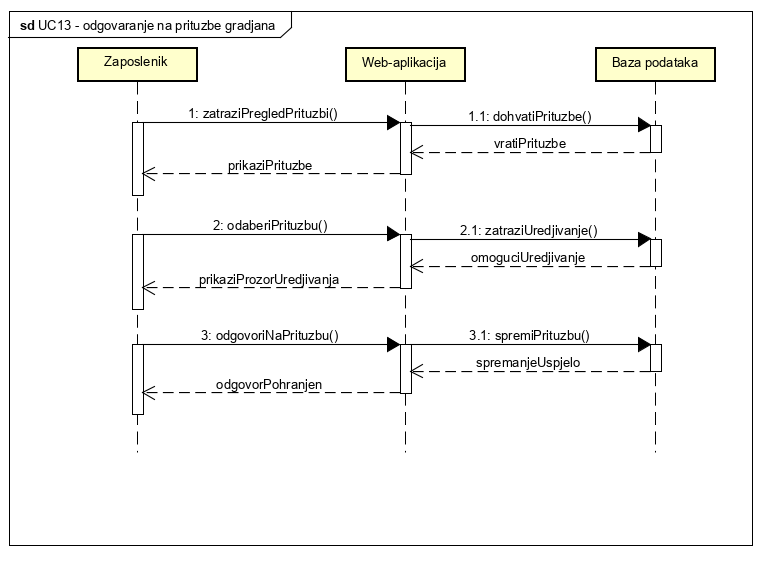
\includegraphics[width=1\linewidth]{dijagrami/uc13seq}
					\caption{Sekvencijski dijagram za UC13}
					\label{fig:uc13seq}
				\end{figure}
			\newpage
			\noindent {\textbf{Obrazac uporabe UC16 - Izmjena termina odvoza}}
			\\
			
			\textmd{\textmd}{Zaposlenik odabire lokaciju za koju mu baza podataka daje informacije. Zatim, zaposlenik mijenja termin odvoza otpada za navedenu lokacija što se ažurira u bazi podataka i postaje vidljivo svim korisnicima web-aplikacije.
				
			 }
		
			\begin{figure}[H]
				\centering
				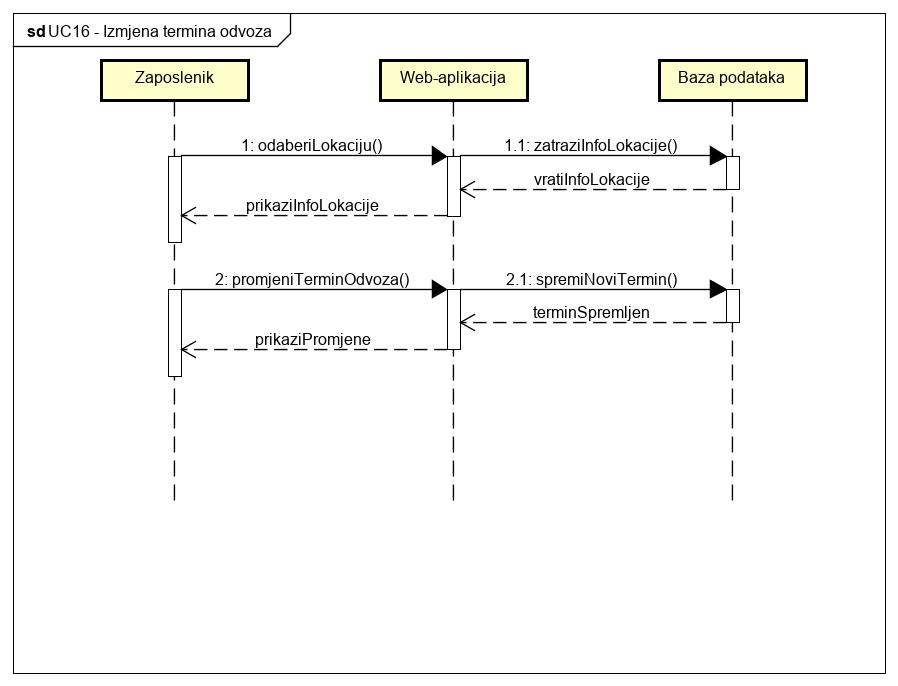
\includegraphics[width=1\linewidth]{dijagrami/uc16seq}
				\caption{Sekvencijski dijagram za UC16}
				\label{fig:uc16seq}
			\end{figure}
			
			\newpage
			
					
		\section{Ostali zahtjevi}
		
		\begin{itemize}
			
			\item Informacije o uslugama tvrtke bit će ažurirane
			\item Sigurnost rada u sustavu osigurat će se unosom korisničkog imena i lozinke
			\item Ako dođe do pogreške na web stranici na to treba upozoriti korisnika porukom
			\item Svaki događaj u sustavu, čak i ako je neuspješan, treba korisniku dati povratnu poruku.
			\item Sustav treba omogućiti rad više korisnika u stvarnom vremenu
			\item Korisničko sučelje i sustav moraju podržavati hrvatsku abecedu(dijakritičke znakove) pri unosu i prikazu tekstualnoga sadržaja
			\item Izvršavanje dijela programa u kojem se pristupa bazi podataka ne smije trajati duže od nekoliko sekundi
			\item Sustav mora raditi na operativnom sustavu Windows 10
			\item zastoji u radu sustava ne smiju prijeći 5 sekundi dnevno
			\item Sustav treba biti implementiran kao web aplikacija koristeći objektno-orijentirane jezike
			\item Neispravno korištenje korisničkim sučelja ne smije narušiti funkcionalnost i rad sustava
			\item Sustav treba biti jednostavan za korištenje, korisnici se moraju znati koristiti sučelje bez opširnih uputa
			\item Nadogradnja sustava ne smije narušavati postojeće funkcionalnosti sustava
			\item Veza s bazom podataka mora biti kvalitetno zaštićena, brza i otporna na vanjske greške
			\item Pristup sustavu mora biti omogućen iz javne mreže pomoću HTTP.
						
		\end{itemize}
			 
			 
			 
	